% Archivo generado automáticamente con los problemas
\section*{Problems}
Sección: 5_Cross_sections_and_decay_rates
Páginas: 86-87
Contenido:
5.1 Show that the differential cross section for 2 →2 scattering with pμ
i + pμ
A →
pμ
f + pμ
B in the rest frame of particle A can be written as
dσ
dΩ =
1
64π2mA
EB + Ef
1 −|⃗pi|
|⃗pf| cos θ
−1 |⃗pf|
|⃗pi| |M|2 ,
(5.54)
where θ is the angle between ⃗pi and ⃗pf, EB =

(⃗pf −⃗pi)2 + m2
B and Ef =

⃗p 2
f + m2
f.

5.2 Show that dΠLIPS is Lorentz invariant and verify Eq. (5.21).

5.3 A muon decays to an electron, an electron neutrino and a muon neutrino, μ−→
e−νμνe. The matrix element for this process, ingoring the electron and neutrino
masses, is given by |M|2 = 32G2
F (m2 −2mE)mE, where m is the mass of the
muon and E is the energy of the outgoing νe. GF = 1.166 × 10−5 GeV−2 is the
Fermi constant.
(a) Perform the integral over dΠLIPS to show that the decay rate is
Γ = G2
F m5
192π3 .
(5.55)
(b) Compare your result to the observed values m = 106 MeV and τ = Γ−1 =
2.20 μs. How big is the discrepancy as a percentage? What might account for
the discrepancy?

5.4 Repeat the e+e−→μ+μ−calculation in Section 5.3 using circular polarizations.

5.5 One of the most important scattering experiments ever was Rutherford’s gold foil
experiment. Rutherford scattering is αN →αN, where N is some atomic nucleus
and α is an α-particle (helium nucleus). It is an almost identical process to Coulomb
scattering (e−p+ →e−p+).
(a) Look up or calculate the classical Rutherford scattering cross section. What
assumptions go into its derivation?
(b) We showed that the quantum mechanical cross section for Coulomb scattering
in Eq. (5.41) follows either from the Born approximation or from quantum field
theory. Start from the formula for Coulomb scattering and make the appropriate
replacements for αN scattering.
(c) Draw the Feynman diagram for Rutherford scattering. What is the momentum
of the virtual photon, kμ, in terms of the scattering angle and the energy of the
incoming α-particle?
68
Cross sections and decay rates
(d) Substitute in for k4 and rewrite the cross section in terms of the kinetic energy
of the α-particle. Show that Rutherford’s classical formula is reproduced.
(e) Why are the classical and quantum answers the same? Could you have known
this ahead of time?
(f) Would the cross section for e−e−→e−e−also be given by the Coulomb
scattering cross section?

5.6 In Section 5.3 we found that the e+e−→μ+μ−cross section had the form dσ
dΩ =
e4
64π2E2
CM (1 + cos2θ) in the center-of-mass frame.
(a) Work out the Lorentz-invariant quantities s = (pe+ + pe−)2, t = (pμ−−pe−)2
and
u = (pμ+ −pe−)2
in
terms
of
ECM
and
cos θ
(still
assuming
mμ = me = 0).
(b) Derive a relationship between s, t and u.
(c) Rewrite dσ
dΩ in terms of s, t and u.
(d) Now assume mμ and me are non-zero. Derive a relationship between s, t and
u and the masses.

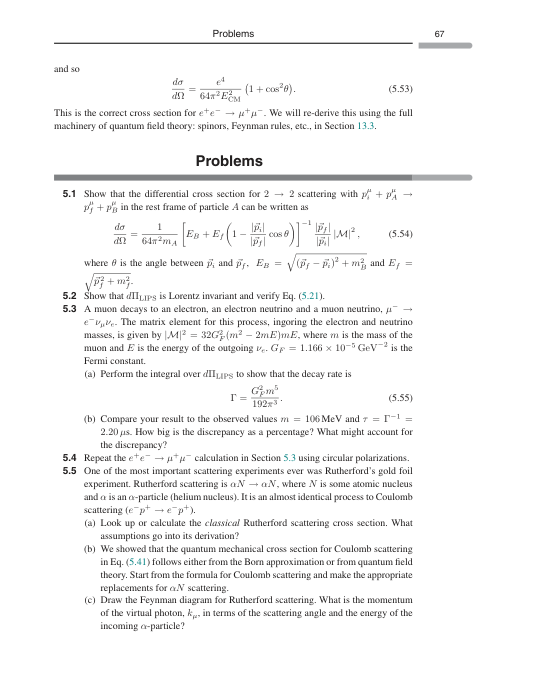
\includegraphics{./figs/5_Cross_sections_and_decay_rates_page_87.png}

---

